\section{Neuromodulation}
In living organisms, neuromodulators are neuropeptides or small molecules, such as dopamine and
serotonin. The production of these substances within the cell is controlled by
gene regulatory networks. Neuromodulators change the behavior of neural networks
within individual neurons, amongst neighboring neurons, or throughout the entire
network. Neuromodulation has been found to be pervasive throughout the brain,
and can have drastic consequences on the behavior of neurons and neuronal
circuits \cite{Destexhe2004,Marder2012,Marder2002}. A particularly applicable
example in the realm of robotics is the neuromodulation of motor signals
produced by central pattern generators in the brain and spinal cord
\cite{Katz1995}. It has been found that neuromodulators tune and synchronize
neuromuscular signals \cite{Zhurov2006}.

We have already noted that the temporal difference learning algorithm for error
prediction has been observed in neural substrates \cite{Schultz1993}.
Dopamine neurons of the ventral tegmental area (VTA) and substantia nigra
exhibit this error predictive behavior. The dopamine system is itself a 
neuromodulatory system. While the temporal difference learning algorithm
extends ideas of reward processing to engineering, there are models of
the dopamine system with closer ties to biology \cite{Montague1996}. These
models also confirm the error predictive behavior found in the brain for a
variety of physiological data including reaction-time and spatial-choice
tasks. Dopamine is an important neuromodulator, especially in learning, but
it is but one of many neuromodulatory substances found in the brain. An
extensive review of computational models of neuromodulation can be found in
\cite{Fellous1998}, and some recent models are reviewed in \cite{Marder2012}.
In this study we extend our previous observations on the relationship between evolved neuromodulator-producing
GRNs and learned behaviors \cite{Harrington2013}. 

\subsection{Regulating parameters}
With the intention of focusing on the optimization of neuromodulator GRNs, the physical mechanisms underlying neuromodulation are only loosely used to inspiration and the neuromodulation of learning behaviors was optimized. Neuromodulation has been considered in the context of RL \cite{Doya2002,Schweighofer2003,Doya2008}, but this previous work has not focused on the implications of neuromodulation on problem solving capacity. In this work we utilize the artificial gene regulatory network presented in the previous section to regulate the learning parameters of the SARSA algorithm. Three learning parameters are considered in this work: the learning rate $\alpha$, the discount factor $\gamma$ and the memory depth $\lambda$.

To do so, the GRN uses three inputs that describes the current performance of the agent in the environment. They have been chosen to be problem-independent: one of our goal is to reduce the configuration of our neuromodulation architecture to have minimum changes to applied when the problem changes. The first input describes the duration since the beginning of current episode: the concentration of this first input protein increases when the agent takes too much time to solve the problem or is getting closer to the end of the episode. The concentraction $C_{I_1}(t)$ of this input protein at time step $t$ is calculated as follows:
\begin{equation}
C_{I_1}(t)=e^{-\frac{t^2}{t_{max}^2}}
\end{equation}
where $t_max$ is the expected duration of an episode. The second output protein's concentration $C_{I_2}(t)$ describes the quality of the current sequence of actions in term of rewards, smoothed on 25 steps:
\begin{eqnarray}
C_{I_2}(t)=\frac{\sum\limits_{s=1}^{25}{\Big((25-s)\times q_s(t-1)\Big)}}{\sum\limits_{s=1}^{25}s} \\
\text{with }q_s(t)=
\begin{cases}
1+1000\frac{q.e}{q.q*e.e} & \text{ if} \frac{q.e}{q.q*e.e}>0.4995\\
0 & \text{ otherwise}
\end{cases}\nonumber
\end{eqnarray}
where $e$ is a vector that contains the current possible action rewards and $q$ is a matrix that contains all the state/action rewards encountered by the agent at time step $t$. The aim of this input is to capture the quality of the current state according to the past states the agent has visited. Finally, the third input protein's concentration $C_{I_3}(t)$ informs the GRN about the 25-step smoothed average reward the agent can obtain in its current state:
\begin{equation}
C_{I_3}(t)=\frac{\sum\limits_{s=1}^{24}{\Big((25-s)\times C_{I_3}(t-s)\Big)}+25\times \sum\limits_{r_e\in e}{r_e}}{\sum\limits_{s=1}{25}s}
\end{equation}
where $e$ is the vector of current possible rewards. This input informs the GRN whether or not the agent is stranded within a long-term decreasing reward. 

In addition to these inputs, the GRN uses four output proteins to regulate the learning parameters:
\begin{itemize}
\item the output protein $O_{n}$, which concentration $C_{n}$ normalizes the concentration of other outputs\footnote{This is generally used in regulatory networks to obtain output values in $[0, 1]$.},
\item the output protein $O_{\alpha}$ of concentration $C_{\alpha}$, which provides the value for $\alpha$ to the SARSA algorithm with $\alpha=C_{\alpha}/(C_\alpha+C_{n})$,
\item the output protein $O_\gamma$ of concentration $C_{\gamma}$, which provides the value for $\gamma$ to the SARSA algorithm with $\gamma=C_{\gamma}/(C_\gamma+C_{n})$,
\item the output protein $O_\lambda$ of concentration $c_{\lambda}$, which provides the value for $\lambda$ to the SARSA algorithm with $\lambda=C_{\lambda}/(C_\lambda+C_{n})$.
\end{itemize}

As depicted by figure \ref{fig:GRNSARSA}, the GRN updates SARSA's learning parameters at every time step, before SARSA updates its internal variables and prediction. The GRN returns the learning parameters SARSA uses for its own decision step.

\begin{figure}
\center
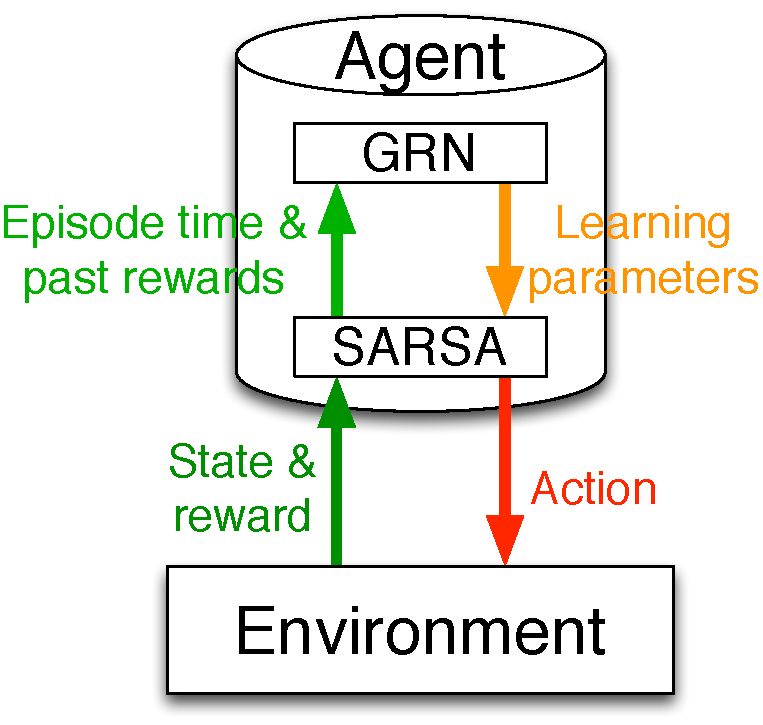
\includegraphics[width=0.7\linewidth]{GRNSARSA.pdf}
\caption{At every time step, SARSA updates the GRN inputs. The GRN returns updated learning parameters that will be used by the SARSA algorithm.}\label{fig:GRNSARSA}
\end{figure}

\subsection{GRN Optimization}
Before using a gene regulatory network for neuromodulation, the network of proteins needs to be optimized. In this paper, we use an adapted genetic algorithm inspired from the NEAT algorithm \cite{stanley2002evolving}. Three features are modified in comparison to a standard genetic algorithm:
\begin{itemize}
\item the \emph{initialization} of the algorithm  - as opposed to initializing with individuals randomly sampled from the complete distribution, only small networks are used in the initial population so as to allow for a more progressive complexification,
\item the \emph{speciation} protects newly appeared solutions by giving them some time to optimize their structures before competing with the whole population, and
\item the \emph{alignment crossover} with the use of a distance metric between proteins to keep subnetwork architecture during the crossover operation.
\end{itemize}
This modified algorithm has been proven to converge faster to better solutions. More details can be find in \cite{cussatblanc2015grneat}.

During its optimization, each GRN is evaluated independently on a given problem with 25 reruns in order to reduce stochasticity impact of the problems on the fitness. The fitness being problem dependent, more explanations will be provided in the experience section. To avoid any memory biais, SARSA is completely resetted before each evaluation. 

!!! Provides GREAT's parameters here !!!





